\section{Analysis of consensus cost}\label{sec:analysis}


\subsection{Round-trip time latency}
In distributed systems communication overhead is much larger than multiprocessing systems. RTTs can reach up to a millisecond in systems in a single data center and can reach hundreds of milliseconds in geographically separated data centers. It is important to understand the behavior of RTTs and the factors that affect its value. Also, it is important to observe how different communication patterns affect observed RTTs. In this section we will show some results on simple experiments to observe the distribution of RTT values. Afterwards, we will analyze the effect of RTT distribution, control patterns, and number of systems on observed latency.

\begin{figure}[ht]
\centering
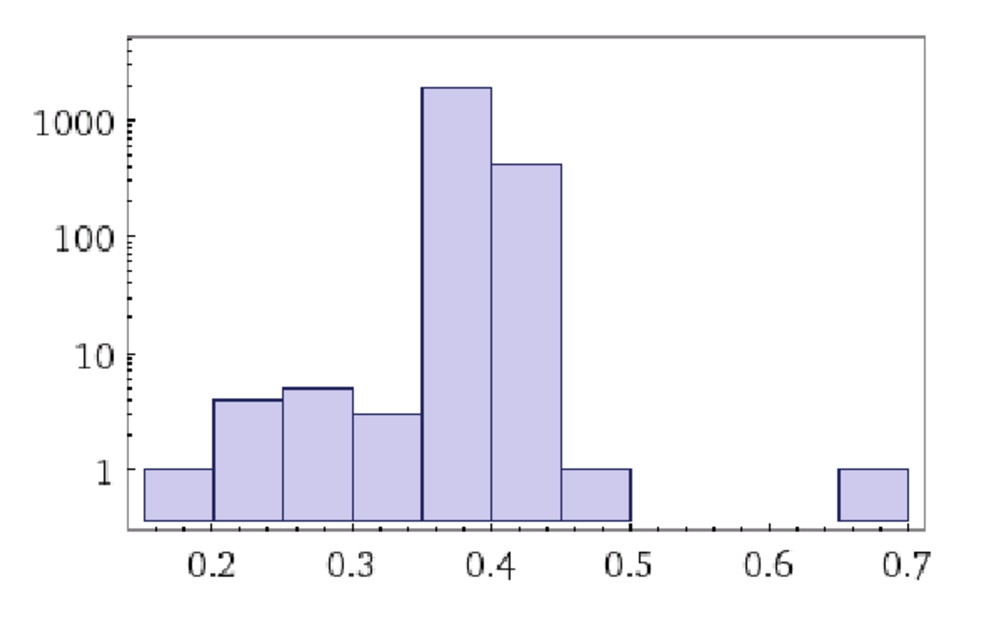
\includegraphics[scale=0.5]{img/rttpdf2.eps}
\caption{probability density function of two machines in the same cluster. X-axis is RTT in milliseconds and y-axis is number of ocurrences}
\label{fig:rttpdf}
\end{figure}

First, we show a probability density function of RTTs between two machines in the same vicinity in Figure~\ref{fig:rttpdf}. It is apparent from the figure that most RTT values are clustered around the average, but also experience variation in values. What is interesting is that obtained results do not resemble traditionally used distributions to approximate them, namely exponential and Gaussian distributions. They are better approximated by a uniform distribution that captures the two largest bars in the displayed histogram.

Simple analysis of a distributed protocol's latency might be deceptive. Lets take 2-Phase commit~(2PC) for example. In this protocol, two rounds of message exchange are required. An observer might naively expect the latency of each operation to be 2 RTTs. However, as we will show in our analysis, this is not the case. The importance of this observation is driven from the fact that coordination systems employ, in one way or another, a consensus or atomic broadcast protocols. These protocol exhibit the same behavior that we will demonstrate analytically in the rest of this section.

\begin{figure}[ht]
\centering
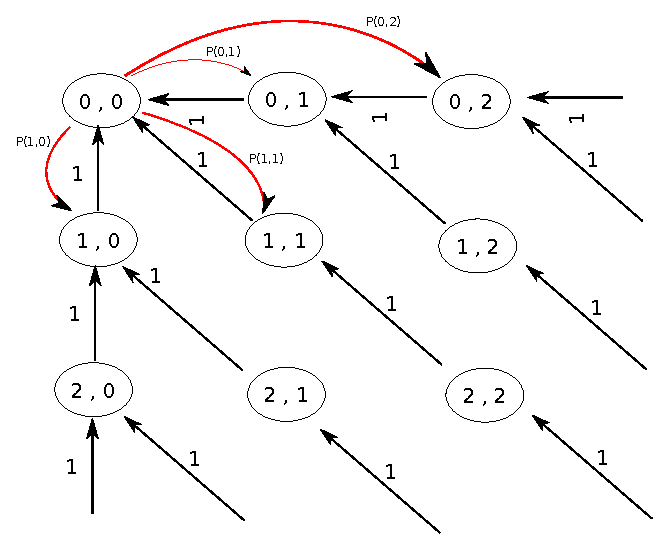
\includegraphics[scale=0.8]{img/markov_general.eps}
\caption{Markov chain to model latency for one master and two slave servers}
\label{fig:markovgeneral}
\end{figure}

Consensus protocols requires the master coordinator to send control messages to associated slave coordinator. Although the average of RTTs when observed with a pair of servers, when we have the master coordinator waiting for more than one slave server the waiting time becomes
\begin{equation}
\label{eq:latency_broadcast}
latency_i = max \{ RTT_i^1, RTT_i^2, \ldots, RTT_i^n \}
\end{equation}
where $latency_i$ is the latency experienced to receive all replies from slaves for request $i$, and $RTT_i^j$ is the RTT for request $i$ for the communication between master and slave $j$. It is clear that the process $latency_i$ has an average larger than $\bar{RTT}$. We model the system as a Markov chain as the one represented in Figure~\ref{fig:markovgeneral} for the case of one master and two slaves. Each state represent the time until receiving the reply of the control message. State $(i, j)$ for example denote that $i$ and $j$ time units are remaining until receiving a reply from slave 1 and 2 respectively. The transition probabilities are described as the following:
\begin{itemize}
\item{A transition from state ($i$, $j$) to state (N($i-1$), N($j-1$)) for all $i$ and $j$ satisfying $i + j > 0$. N(i) returns $i$ if it is positive or zero otherwise.}
\item{A transition from state (0, 0) to state ($i$, $j$) with probability $\psi_i\psi_j$ where $\psi_k$ is the probability distribution of the RTT process.} 
\end{itemize}
This model can be used to reach the real latency of communication on such broadcast systems. To get a sense of the effect of Equation~\ref{eq:latency_broadcast} lets take the cumulative distribution function (cdf) of latency process:
\begin{equation}
latency_{cdf}(x)  = \prod_{i \in N} RTT_i(X \leq x)
\end{equation}
where $latency_{cdf}(x)$ is latency's cdf for a value $x$, $N$ is the set of servers to communicate with, and $RTT_i(X \leq x)$ is the cdf for the process $RTT_i$. Since the value of any cdf is less than or equal to one, multiplying two cdf functions will result in a value smaller than both of them. Therefore, the cumulative distribution function of the latency of waiting for replies of a broadcast message is at least as bad as the slowest RTT process.

\subsection{Consensus latency}
Zookeeper uses paxos algorithm for consensus management. In paxos, when a proposal is broadcasted, the proposal does not wait for all followers to reply. Rather, a majority is enough to proceed with committing the proposal. This is important to notice when applying our findings from the previous subsection. Thus, Equation~\ref{eq:latency_broadcast} for describing the latency process becomes:
\begin{equation}
latency^p_i = max \{ RTT_{fastest majority} \}
\end{equation}
where $latency^p_i$ is latency of each broadcast of paxos, and $RTT_{fastest majority}$ is the set of $\lceil\frac{n + 1}{2}\rceil $ fastest nodes RTTs for iteration $i$.

\subsection{Synchronization primitives latency}
We will consider the latency of queue locks and TAS. For queue locks, a simple M/M/1 queue model can be used to characterize the system. Having $\lambda$ as the interarrival rate of requests to enter the critical section and $\mu$ as the service rate, hence inverse of the time spent inside the critical section. We assume that both interarrival and service times are exponentially distributed. In that case the average number of concurrent lock requests, $\bar{N}$ is:
\begin{equation}
\bar{N} = \frac{\rho}{1 - \rho}
\end{equation}
where $\rho$ is the ratio of interarrival to service time. Using Little's theorem we can find an expression of average time spent in the system (time from acquiring until releasing the lock)
\begin{equation}
\label{eq:wait}
W = \frac{\bar{N}}{\lambda} = \frac{1}{\mu - \lambda}
\end{equation}
where $W$ is the total wait time in the system.

TAS can be modeled as a M/M/1/$\infty$/$\infty$/SIRO queue. This is identical to M/M/1 queue with one difference; queueing discipline is SIRO~(Service In Random Order) rather FIFO~(First In First Out). The calculations that lead to Equation~\ref{eq:wait} is not affected by the queueing discipline. Thus, $W_{FIFO} = W_{SIRO}$.

\subsection{Overall system}
We laid the building blocks of modeling the whole synchronization system above. Now, we will put them together to see the big picture and model the latency of the system. Each client go through the following stages for each lock request:
\begin{itemize}
\item{\emph{Connection establishment}: this is described by the RTT process between the user and cluster, \emph{i.e.}, $RTT_{user-to-server}$.}
\item{\emph{Acquiring the lock}: this includes the time for executing necessary operations to try acquiring the lock (before actually acquiring it) and to establish the acquirement of the lock (before entering the critical section). We will denote those two as $T_{pre-acquire}$, and $T_{post_acquire}$. Note that both are functions of $RTT_{user-to-server}$ and $latency^p$.}
\item{\emph{Waiting for the lock}: The time spent waiting for the lock to be available, including the current user holding the lock and other users that will hold the lock while you are waiting. This period is usually between trying acquiring the lock and establishing the acquirement of the lock. The wait time is described in Equation~\ref{eq:wait} as $W$.}
\item{\emph{Time in critical section}: This is the time spent holding the lock. The average of this time is $\frac{1}{\mu}$, where $\mu$ is the rate of processing requests in mutual exclusion block.}
\item{\emph{Releasing the lock}: The time required to release the lock. Our implementations release the lock by asynchronously deleting a file representing holding the lock, denoted as $T(delete_{async})$. }
\item{\emph{Closing the connection}: time required to close the connection, denoted as $T(close)$. }
\end{itemize}
Putting all these components together we can arrive to an expression of synchronization primitives latency with respect to the user. Each of these aspects requires separate treatment to minimize its latency. Further, different contention and network conditions will dictate which primitive to be used, since different ones have different influences on each component. This question is what we will tackle in the next section.











